\newpage
\section{Text-to-Tree transformation}
\genHeader

As we shall see in a moment, libraries and shelves correspond to a folder structure while the contents for a single dictionary are specified in a file.
Figure \ref{fig:moca-4-Tokens} depicts a small sample of the textual syntax used to specify a dictionary. 

\begin{figure}[!htbp]
\begin{center}
 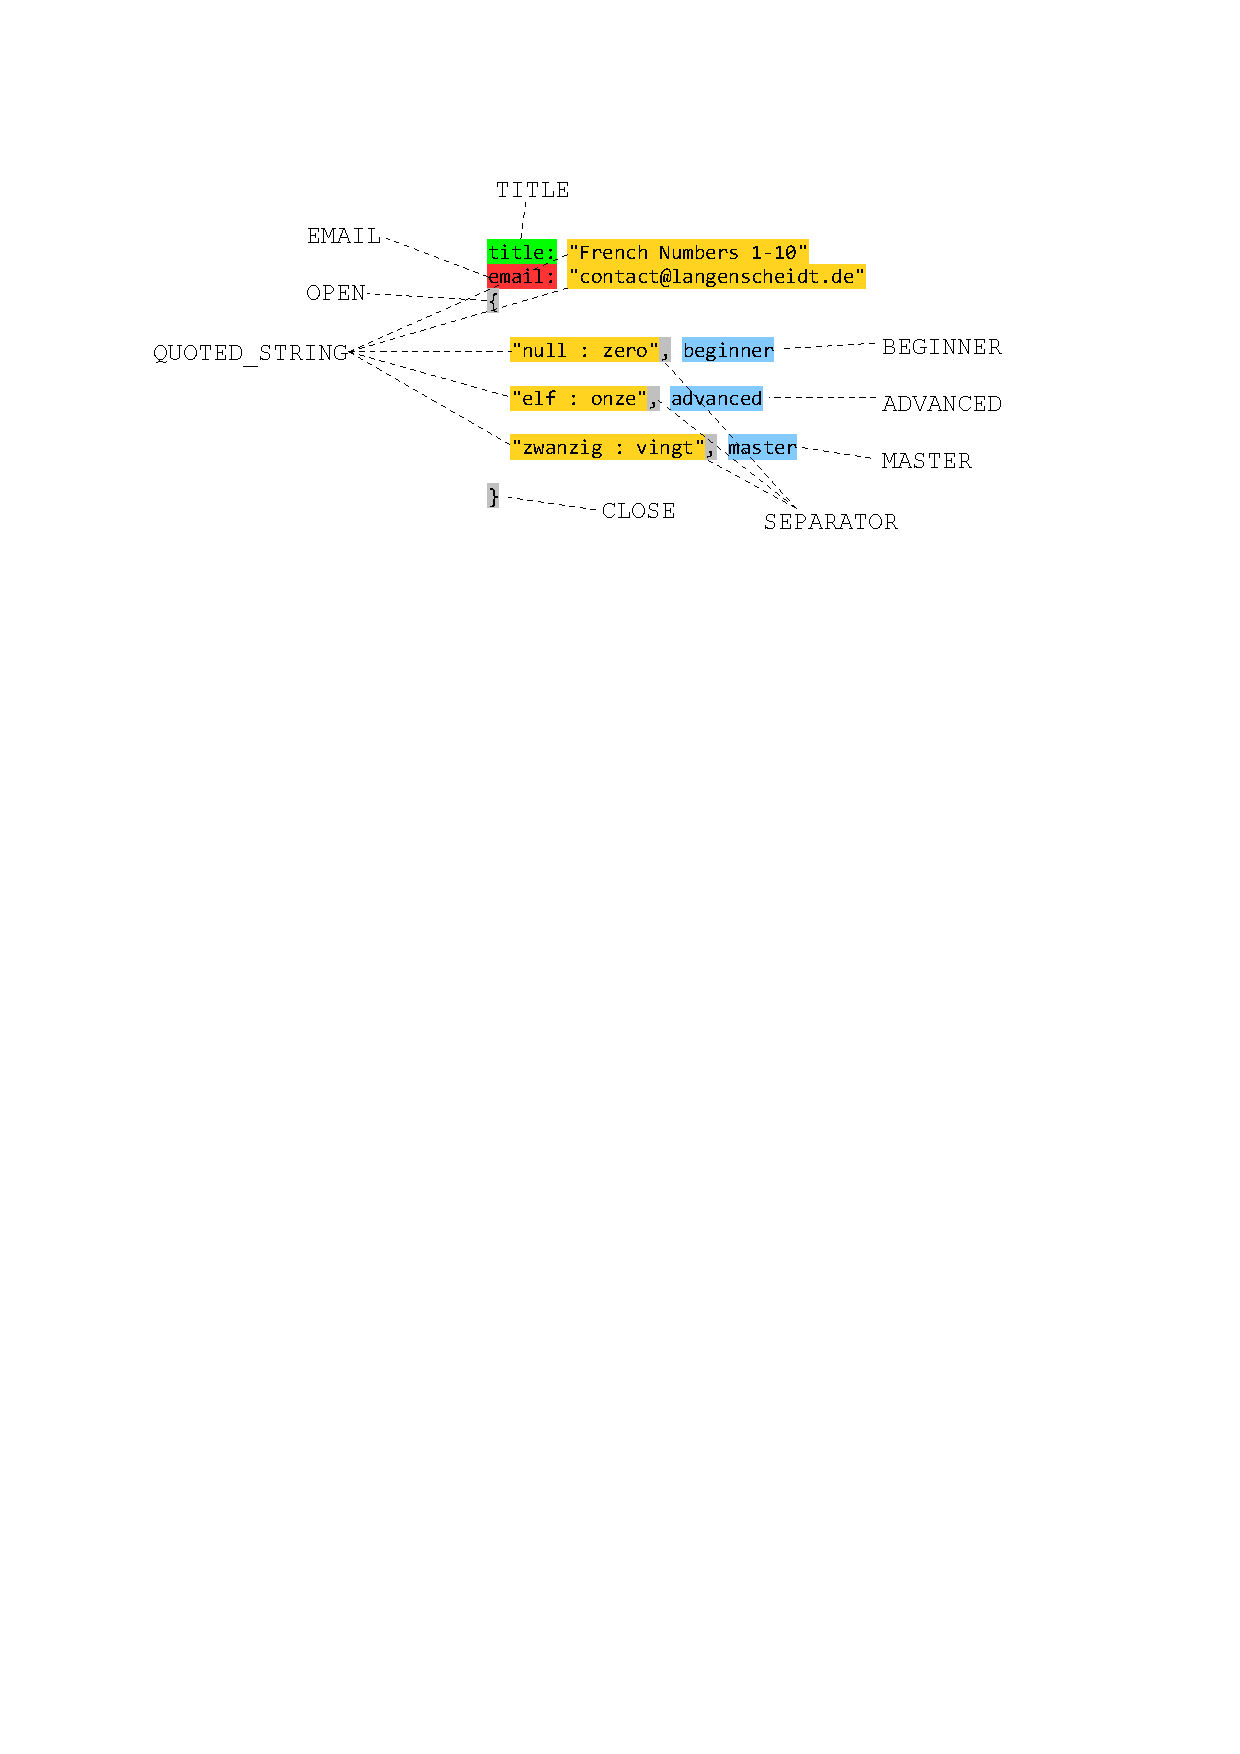
\includegraphics[width=0.7\textwidth]{4-tokens}
  \caption{Identified tokens in a dictionary file \update}
  \label{fig:moca-4-Tokens}
\end{center}
\end{figure}

On the way to an instance model of our dictionary metamodel, the very first step is to create nice \emph{chunks} of characters. This step is called
\emph{lexing} and it simplifies the actual comprehension of the complete text. Interestingly human beings actually comprehend text in a similar manner, one
recognizes whole words without ``seeing'' every individual character. This is the reason why you can siltl raed tihs sneentce alsomt eforftlsesly. A lexer
recognizes these chunks or \emph{tokens} and passes them on as a token stream to the \emph{parser} that does the actual work of recognizing complex
hierarchical and recursive structures.
   
To recognize the tokens as indicated in Fig.~\ref{fig:moca-4-Tokens}, \texttt{ANTLR} can automatically generate a lexer in Java from a compact specification.
This is actually a DSL for lexing and is explained in detail in \cite{ANTLR}. If you are unfamiliar with EBNF, and have feel you may have problems understanding
the lexer grammar, we suggest going through the documentation on on \url{www.antlr.org}, or reading the relevant chapters in \cite{ANTLR}. Otherwise, let's
complete the \emph{lexer} and \texttt{parser} grammars that will handle our project instances.

\begin{itemize}
  
\item[$\blacktriangleright$] Navigate to ``DictionaryCodeAdapter/src/org.moflon.moca.dictionary.parser" and edit \texttt{DictionaryLexer.g} until it closely
resembles Fig.~\ref{eclipse:dictionaryLexer}. Don't forget to add the \texttt{import org.moflon.moca.MocaUtil} statement to the header, and be vigilant to avoid
any typos and mistakes! Save to compile the file, and ensure no errors persist before proceeding.

\end{itemize}
\newpage

\begin{figure}[!htbp]
\begin{center}
  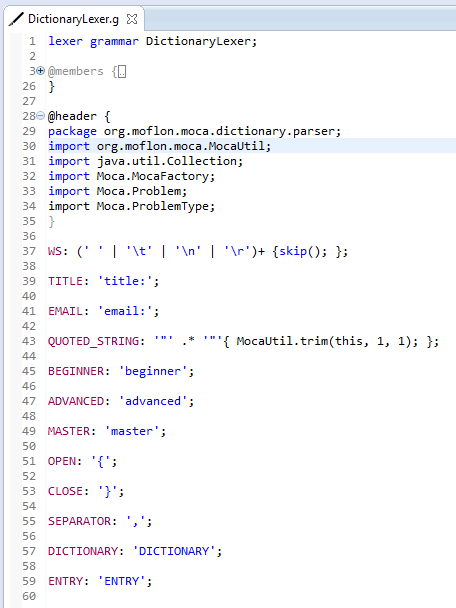
\includegraphics[width=0.7\textwidth]{eclipse_dictionaryLexer}
  \caption{Lexer grammar}
  \label{eclipse:dictionaryLexer}
\end{center}
\end{figure}

With our lexer, we can now complete the next step of forming its stream of tokens into a \emph{tree}. In this context, a \emph{tree} is an acyclic,
hierarchical, recursive structure (as depicted in Fig.~\ref{eclipse:dictLexer}). Depending on what the tree is to be used for, it can be organized much
differently with extra \emph{structural} nodes such as \texttt{DICTIONARY} or \texttt{ENTRY} which were not present in the textual syntax, which can be used to
give additional meaning to the tree.

\begin{figure}[htp]
\begin{center}
 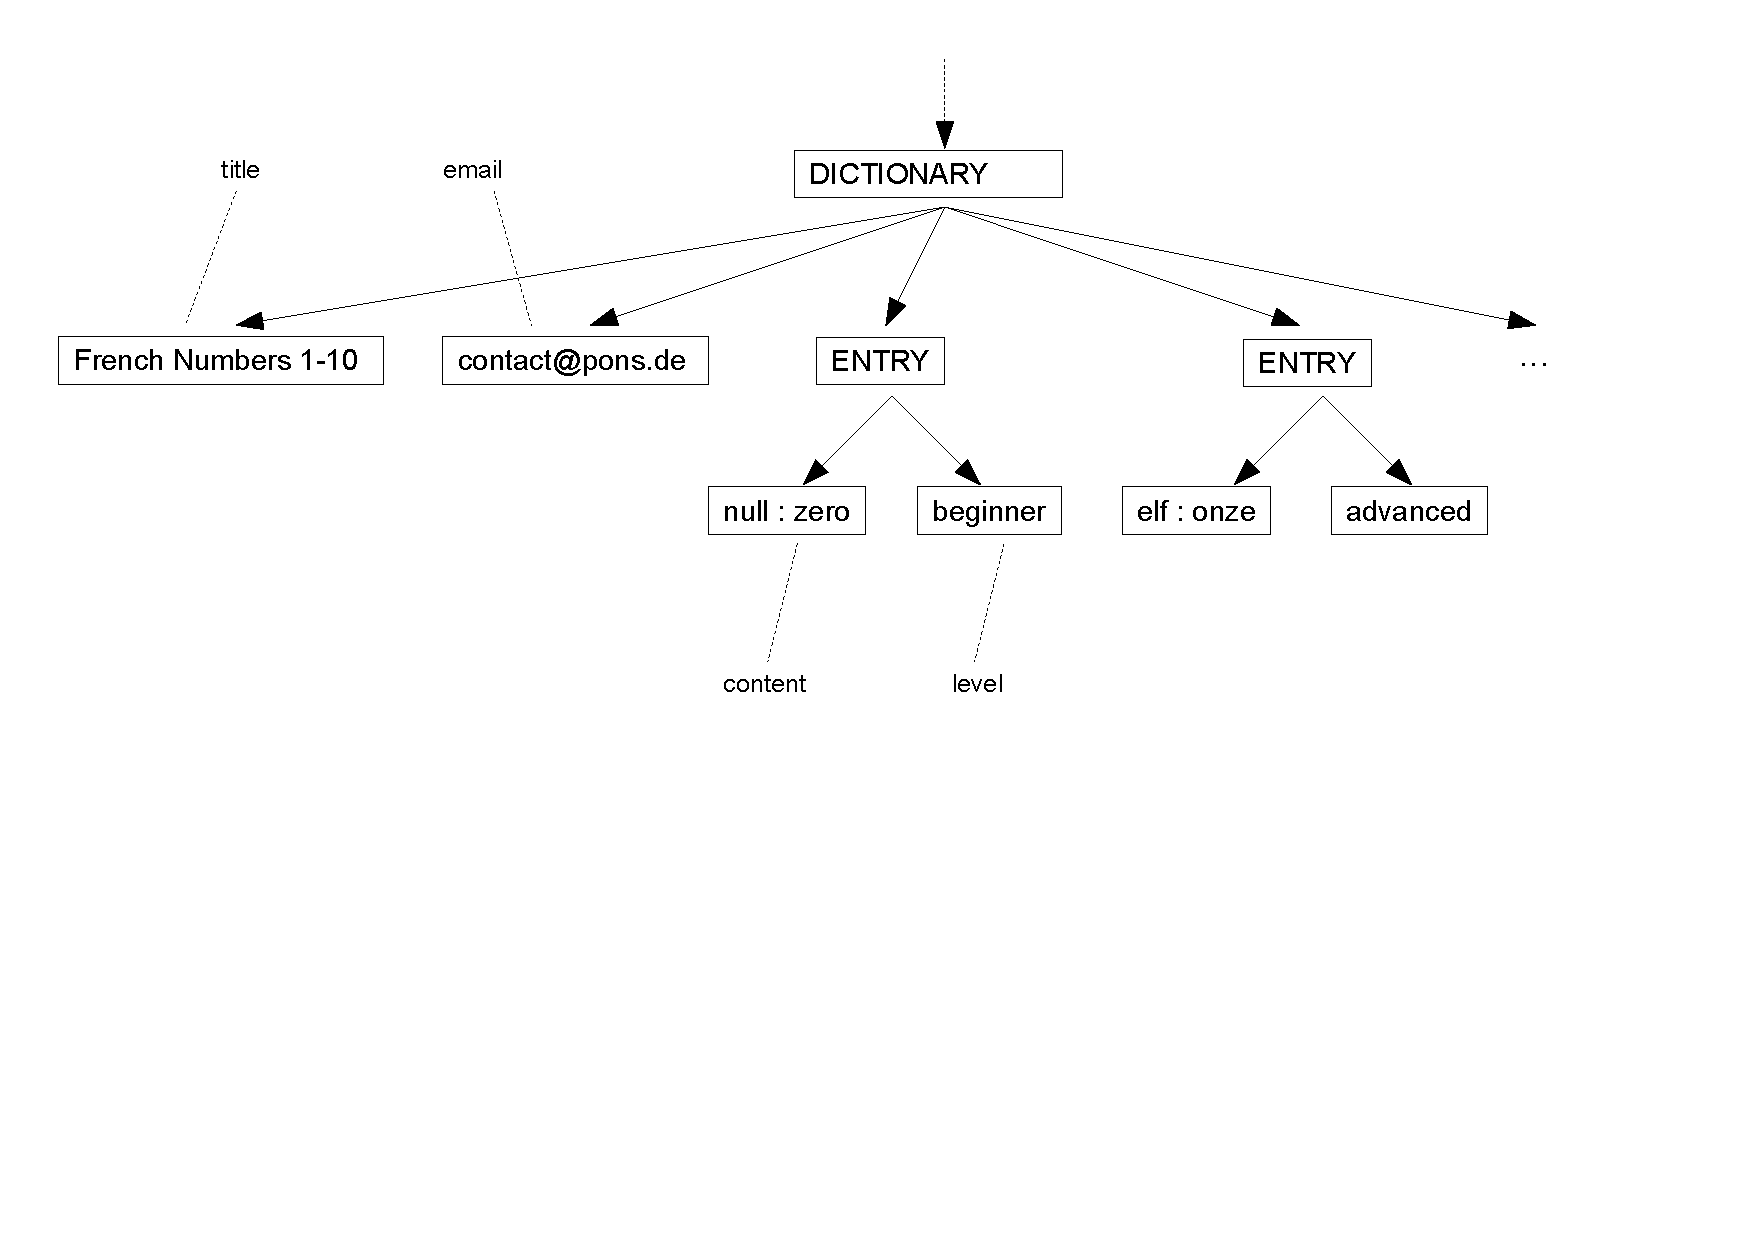
\includegraphics[width=\textwidth]{5-tree}
  \caption{MocaTree structure}
  \label{eclipse:dictLexer}
\end{center}
\end{figure}

\begin{itemize}

\item[$\blacktriangleright$] Open and edit \texttt{DictionaryParser.g} from the same package until it closely resembles Fig.~\ref{eclipse:dictParser}. As with
the lexer, avoid typos and mistakes and ensure it compiles before proceeding.

\end{itemize}

\begin{figure}[!htbp]
\begin{center}
 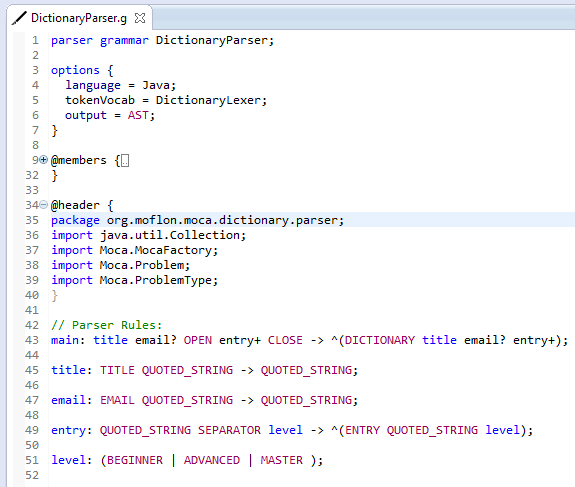
\includegraphics[width=0.9\textwidth]{eclipse_dictionaryParser}
  \caption{Parser grammar}
  \label{eclipse:dictParser}
\end{center}
\end{figure}

\newpage

You'll notice that the parser grammar is extremely similar to the lexer grammar, save for some \emph{parser actions} following the \texttt{`->'} symbol. These
actions order the construction of the tree. Using this simple tree language, one can (1) abstract from tokens like \texttt{`\{'} or \texttt{`\}'}, which are
just \emph{syntactical noise}\footnote{Irrelevant content for our model.} and (2) enrich the tree with structural nodes like \texttt{ENTRY}, which add explicit
structure to the tree. Refer to \cite{ANTLR} and online resources for detailed explanations on the syntax and semantics of the parser grammar supported by
\texttt{ANTLR}.

\begin{itemize}


\item[$\blacktriangleright$] Before taking our lexer and parser out for a spin, navigate to ``src/org.moflon.tie" and open \texttt{TGGMain.java}. If everything
has been generated properly so far, it should resemble Fig.~\ref{eclipse:defaultTGGMain}.

\begin{figure}[!htbp]
\begin{center}
 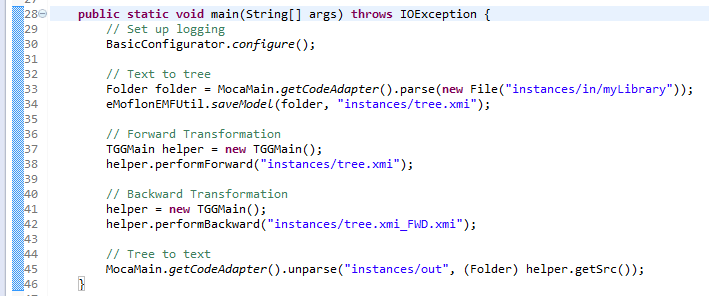
\includegraphics[width=0.9\textwidth]{eclipse_TGGMainDefault}
  \caption{Deafult TGG}
  \label{eclipse:defaultTGGMain}
\end{center}
\end{figure}

\item[$\blacktriangleright$] You can see that this method is the driver for the program, executing each of the four pieces required for a full forward and
backwards transformation. It begins the process by parsing the contents of the \texttt{myLibrary} folder, which we haven't created yet. 

\vspace{0.5cm}

In a nutshell, each folder is taken as a root of a tree and the folder and file structure is reflected as a hierarchy of (children) nodes in the tree.
For each file, the framework searches for a registered parser that is responsible for the particular file, passes the content on to the parser and plugs in the
tree from the parser as a single subtree of the corresponding file node in the overall tree.  

\newpage

\item[$\blacktriangleright$] We're not concerned with the final output right now however, so comment out line 45, which calls the unparser to generate an output
directory structure. We will define this model-to-text unparser a bit later. It should be noted for future reference that if decided to experiment with multiple
libraries (such as one for languages and one for sciences), this is the file where you'll need to update the appropriate information.

\item[$\blacktriangleright$] The final step is now to prepare some input for the framework. Navigate to ``DictionaryCodeAdapter/instances/in'' and create the
directory structure depicted in Fig.~\ref{eclipse:textDirectory}. You can create the \texttt{dictionary} files by right-clicking its parent folder, going to
``new/File" and simply appending \texttt{.dictionary} to the end of the name. 

\item[$\blacktriangleright$] Complete each of the four \texttt{.dictionary} files with the contents in Table~\ref{moca-inputdata}.\footnote{Please do not copy
and paste this data as it your .pdf reader may add some invisible characters to the file that MOSL will not detect}

\begin{figure}[htp]
\begin{center}
  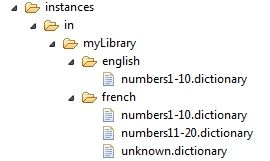
\includegraphics[width=0.5\textwidth]{inputData}
  \caption{Input directory structure.}
  \label{eclipse:textDirectory}
\end{center}
\end{figure}

\item[$\blacktriangleright$] As you can see, this creates a single library split into two languages, each containing unique dictionaries. Reviewing
Fig.~\ref{eclipse:dictParser}, you can see that the structure of these files conform to the parser's \texttt{main} command: it first lists the dictionary's
\texttt{title}, may or may not contain a \texttt{author}, and contains all \texttt{entry} elements between the \texttt{OPEN} and \texttt{CLOSE} brackets.

\end{itemize}

\newpage

\begin{table}
\begin{tabular}{p{6cm} p{6cm} }
\footnotesize
\textbf{english/numbers1-10.dictionary:}
\begin{verbatim}
title: "numbers1-10"
email: "contact@langenscheidt.de"	
{
  "null : zero", beginner
  "eins : one", beginner
  "zwei : two", beginner
  "drei : three", beginner
  "vier : four", beginner
  "fuenf : five", beginner
  "sechs : six", beginner
  "sieben : seven", beginner
  "acht : eight", beginner
  "neun : nine", beginner
  "zehn : ten", beginner 
}
\end{verbatim} 

\footnotesize
\textbf{french/numbers11-20.dictionary:}
\begin{verbatim}
title: "numbers11-20"
email: "contact@pons.de"	
{
  "elf : onze", advanced
  "zwoelf : douze", advanced
  "dreizehn : treize", advanced
  "vierzehn : quatorze", advanced
  "fuenfzehn : quinze", advanced
  "sechzehn : seize", master
  "siebzehn : dix-sept", master
  "achtzehn : dix-huit", master
  "neunzehn : dix-neuf", master
  "zwanzig : vingt", master
}
\end{verbatim}
&

\footnotesize
\textbf{french/numbers1-10.dictionary:}
\begin{verbatim}   
title: "numbers1-10"
email: "contact@pons.de"	
{
  "null : zero", beginner
  "eins : un/une", beginner
  "zwei : deux", beginner
  "drei : trois", beginner
  "vier : quatre", beginner
  "fuenf : cinq", beginner
  "sechs : six", beginner
  "sieben : sept", beginner
  "acht : huit", beginner
  "neun : neuf", beginner
  "zehn : dix", beginner 
}
\end{verbatim}

\footnotesize
\textbf{french/unknown.dictionary:}
\begin{verbatim}
title: "unknown"
{
	"unbekannt : unknown", beginner
}
\end{verbatim}
  \\
\end{tabular}   
\caption{Input files containing dictionaries.}
\label{moca-inputdata}

\end{table}   

\begin{enumerate}


\item[$\blacktriangleright$] Before saving each dictionary file, double check and confirm that you have not missed any characters (such as colons or
commans) -- parsing will not succeed to the files do not perfectly conform to the lexer. 

\item[$\blacktriangleright$] One finished, right click on \texttt{TGGMain} and navigate to ``Run As / Java Application'' in the context menu. Refresh the
\texttt{instances} folder. Several models have been created (Fig.~\ref{eclipse:postParse})! 

\begin{figure}[!htbp]
\begin{center}
 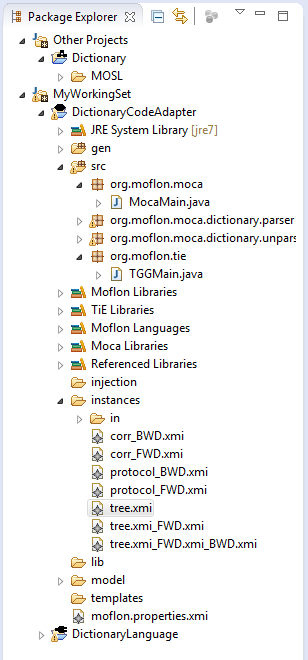
\includegraphics[width=0.4\textwidth]{eclipse_explorerPostGeneration}
  \caption{new tgg file generation result}
  \label{eclipse:postParse}
\end{center}
\end{figure} 

\item[$\blacktriangleright$] To explain, \texttt{tree.xmi} is the model generated directly from the \texttt{myLibrary} directory. \texttt{tree.xmi\_FWD.xmi} is
the \texttt{Dictionary} result of the forward generation which also produced \texttt{corrFWD.xmi} and \texttt{protocol\_FWD.xmi}. This should be ?? EMPTY ??.

\item[$\blacktriangleright$] As you can probably assume, the backwards transformation generated \texttt{corrBWD.xmi}, \texttt{protocolBWD.xmi}, and
\texttt{tree.xmi\_FWD.xmi\_BWD.xmi}, which will eventually resemble the original \texttt{tree.xmi} model.

\item[$\blacktriangleright$] Open the generated \texttt{tree} model. \update EXPLAIN THE NODES HERE?
compare the contents to Fig.~\ref{eclipse:treeResult}. At this point, you can reflect on the structure of the tree and note the directory structure, file nodes
and the subtrees from the parser. This file is important to understand; The directory structure is transformed to a corresponding hierarchy of \texttt{Folders}
and \texttt{Files}. The actual \emph{textual content} of each file is then transformed to a subtree using a registered, suitable parser. The resulting subtree
from the parser is then plugged into the tree by setting its root as the single child node of a \texttt{File}.

\item[$\blacktriangleright$] \update Mention that the reason why so many files were created were to go from text to model, model to text, we need a tree as a
middle man??

\end{enumerate}

\begin{figure}[!htbp]
\begin{center}
 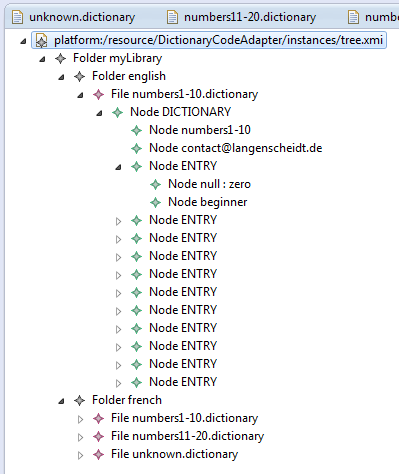
\includegraphics[width=0.6\textwidth]{eclipse_textParsingGeneration}
  \caption{MocaTree created by the framework using our parser}
  \label{eclipse:treeResult}
\end{center}
\end{figure}

If everything worked out, well done! You've just completed the first step in the transformation: Text to tree. Now, to finish the forwards transformation,
we'll need to go from the tree to a model. It follows that it will end with model to tree, then tree to text. You now have a nicely structured tree that we'll
be able to use with TGGs and transform in a few simple steps into an actual instance of our \texttt{Dictionary} metamodel.
